\section{Introduction}\label{sec:intro}

Metapopulation models, in which spatially distinct sub-populations are connected by host movement, are among the most widely used tools for understanding regional infectious disease dynamics and for generating the forecasts that support public health decisions~\citep{grenfell_metapopulation_1997,keeling_modeling_2011,riley_large-scale_2007,rohani_opposite_1999}. 
When SARS-CoV-2 emerged, these models proved instrumental in projecting disease burden and evaluating intervention strategies across geographic scales from counties to nations~\citep{pei_differential_2020,cramer_evaluation_2022,bertozzi_challenges_2020}. 
At the same time, the pandemic exposed challenges with building spatial models, adapting them to new settings, and providing reproducible tests of hypotheses.
In practice, most researchers build bespoke implementations of metapopulation models in which assumptions about transmission, host movement, and geographic structure are intertwined throughout custom code bases, making it difficult to compare alternative model formulations, adapt models to new pathogens, or even reproduce published analyses~\citep{willem_lessons_2017,pollett_recommended_2021}.
While new software has emerged to enable flexible modeling, no existing environment supports the full life cycle of a spatial modeling study within a modular, pathogen-agnostic framework that provides choices of model structures, advanced statistical inference algorithms, and customizable forecasting.

Spatial epidemiological models have suffered from issues with both reproducibility and comparability. 
A pivotal study could only completely reproduce 4 of 100 randomly sampled COVID-19 modeling studies~\citep{henderson_reproducibility_2024}, a problem now recognized widely enough to have prompted a 22-element framework for reproducibility in computational epidemiology that current studies rarely satisfy~\citep{pokutnaya_implementation_2023}. 
Our own systematic review of 109 spatial epidemiological studies of COVID-19 found that only 30.6\% provided accessible code~\citep{oshinubi_systematic_2026}.

Failures in the reproducibility of metapopulation models compound a deeper comparability problem. 
Metapopulation models have high-dimensional state spaces and complex spatial interdependencies that necessitate sophisticated inference algorithms such as particle filters or ensemble Kalman filters~\citep{king_statistical_2016,ganyani_simulation_2021,ionides_iterated_2024}, yet implementing these methods requires substantial expertise and custom code for each model structure~\citep{asfaw_tutorial_2024,ning_iterated_2023,funk_choices_2020}. 
It is therefore fundamentally difficult to systematically isolate which modeling choices drive differences in forecast accuracy~\citep{shea_harnessing_2020,reich_collaborative_2022,cdc_flusight_2026,loo_us_2024}. 
To systematically understand which modeling structures work in which geographic regions, we need to decompose the spatial modeling problem into modular components, from transmission and disease processes to movement patterns to geographic context, which can be explored together and in isolation~\citep{bicker_memilio_2026,lemaitre_flepimop_2024,oshinubi_systematic_2026}.
And we therefore need software that implements this abstraction to encapsulate the full modeling and forecasting workflow, from data acquisition through model specification, calibration, and probabilistic prediction, as a customizable but reproducible pipeline~\citep{lutz_applying_2019,moran_future_2025,birrell_evidence_2018}.

Existing software addresses individual components of this metapopulation modeling workflow, but none spans it in full (Table~\ref{tab:comparison}). 
On one hand, there are statistical inference toolkits that are powerful and implement broad collections of fitting algorithms for partially observed Markov processes, such as \texttt{pomp} and its spatiotemporal extension \texttt{spatPomp}~\citep{king_statistical_2016,ionides_iterated_2024,asfaw_tutorial_2024}, the \texttt{odin2}/\texttt{dust2}/\texttt{monty} stack~\citep{fitzjohn_reproducible_2021}, and \texttt{LibBi} with its \texttt{rbi} interface~\citep{murray_bayesian_2015}. 
But these tools are not tailored to epidemiological questions, where every model needs to be hand-coded (e.g, C snippets), and none of the software retrieves common data sets, raising the barrier to entry. 
On the other hand, epidemiology-specific pipelines supply domain-specific infrastructure but most often commit to a single inference strategy, a single model class, or a single type of pathogen (e.g., respiratory viruses). 
For instance, \texttt{FlepiMoP} implements customizable metapopulation compartmental models for directly-transmitted, respiratory diseases, with built-in Bayesian inference scheme, and some essential data sets. 
However, a problem is that movement dynamics are largely constrained by a fixed mixing formulation, such that users cannot specify unique movement dynamics~\citep{lemaitre_flepimop_2024}.  
\texttt{MEmilio} envisions a modular metapopulation model specification, but it has no built-in support for parameter estimation or forecasting~\citep{bicker_memilio_2026}.
We provide a structured, reproducible comparison across the full software landscape (Methods). 
No existing package combines independently exchangeable transmission, movement, and geographic components, automated data acquisition based on time and place of interest, and choices in Bayesian filtering algorithms that estimates time- and space-varying parameters, all feeding a customizable forecasting pipeline (Table~\ref{tab:comparison}). 

Here we introduce \texttt{epymorph}, a Python package that provides a unified, modular framework for specifying, calibrating, and forecasting high-dimensional metapopulation models of disease.
\texttt{epymorph} implements our solution to the design of metapopulation models~\citep{oshinubi_systematic_2026},
where the model is decomposed into three interacting sub-models: an intra-population model (IPM) describing transmission and disease dynamics via a compartment model, including multi-strata structures such as age groups or multi-species (e.g., vector-borne) transmission; a movement model (MM) representing how hosts or vectors move between spatially distinct sub-populations; and a geographic context (GEO) that is automatically linked to data requirements (e.g., sub-population counts, local environmental and demographic features) (Fig.~\ref{fig:architecture}).
Because the components are modular, by changing a single line of code, a user can, for example, deploy a compartmental model in a new geography, or swap a distance-based movement pattern with a commuter model.


% GENERATED by software-lit-search/src/table1_tex.py -- do not hand-edit.
\input{tables/table-1-maintext}

\texttt{epymorph} therefore provides a disease-agnostic, modular framework for designing and testing metapopulation models in a largely automated workflow. 
For U.S.-based studies, \texttt{epymorph} automates the acquisition of Census population data at resolutions from state to census block group, empirical commuting flows, PRISM climate data, and CDC surveillance data, removing the requirement that users be experts in munging diverse data sources. 
Our internal data machinery ensures that model inputs and outputs are harmonized, such that each quantity returned conforms to the study's geographic scope and time frame. 
Importantly, studies outside the United States, or studies wanting to use custom geographic scopes, can still leverage the same modeling, inference, and forecasting machinery, by supplying custom data through the same interface. 
This effectively exposes epymorph's simulation and inference framework to any spatial modeling domain based around compartmental models. 
Compiled models are executed as stochastic simulations and fit to observations using a choice of particle filtering~\citep{gordon_novel_1993,arulampalam_tutorial_2002} or ensemble Kalman filtering~\citep{evensen_ensemble_2003,lal_application_2021,abbas_joint_2025}, accommodating stratified data and multiple simultaneous surveillance streams (e.g., fitting to cases and hospitalizations). 
Fitted models then feed a probabilistic forecasting pipeline that can, for example, simulate the effects
of locally-refined interventions through the forecast window. 


\begin{figure}[t]
\centering
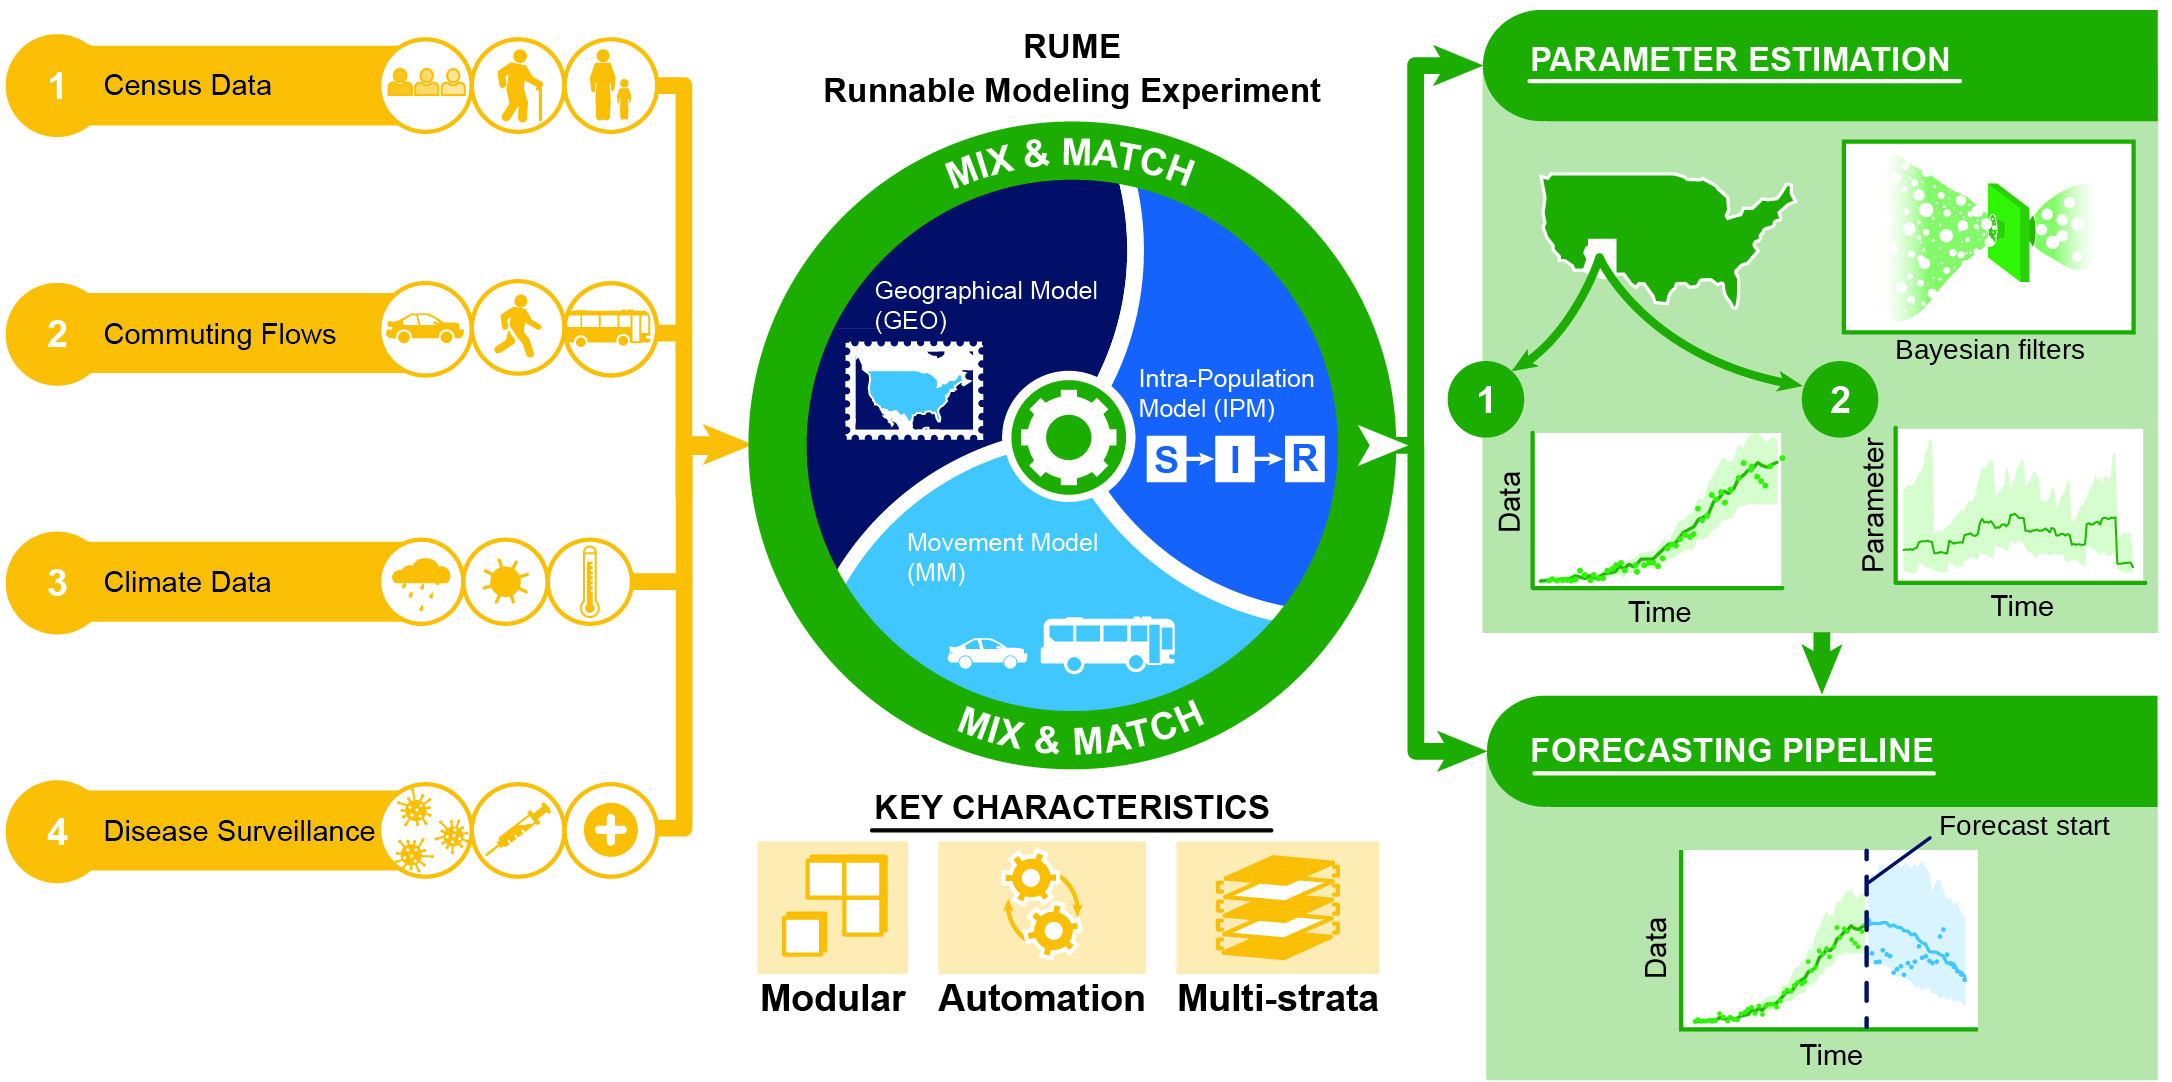
\includegraphics[width=\textwidth]{figures/fig1-epymorph-architecture.jpg}
\caption{\textbf{Architecture of \texttt{epymorph}.} Left: Examples of data (census, commuting flows, climate, and disease surveillance) that are retrieved automatically for a chosen geographic scope by Abstract Data Resource Interface Objects (ADRIOs). Center: the Runnable Modeling Experiment (RUME) combines an intra-population model (IPM), a movement model (MM), and a geographical model (GEO), each of which can be exchanged independently of the others (``mix and match''). Key characteristics of the package are its modularity, the automation of data acquisition, and its support for multi-strata models. Right: the same RUME is passed, without re-specification, to parameter estimation, which returns location-specific fitted trajectories (1) and time-varying parameter estimates (2), and to the forecasting pipeline, which generates probabilistic forecasts from the calibrated ensemble.}
\label{fig:architecture}
\end{figure}


Here we demonstrate our vision of using \texttt{epymorph} for controlled, reproducible hypothesis-testing. 
For two case studies, we compare competing models by running them through the an advanced forecasting pipeline enabled by \texttt{epymorph}.
First, we test whether age-stratification and empirically derived contact mixing improve forecasts of influenza hospitalizations across the United States during the 2025-2026 season. 
Second, we test the roles of spatial resolution and host movement in forecasting SARS-CoV-2 hospitalizations and deaths in three New England states during the 2020-2021 winter wave. 
We find that empirical age-structured contact mixing improves influenza forecasts, increasingly so at longer horizons, whereas for SARS-CoV-2 a coarser State-level model outperforms county-level models at forecasting State-level data, although empirical commuting improves county-level forecasts relative to no movement.
By making model components interchangeable, automating spatial and surveillance data workflows, and exposing multiple inference algorithms through a common interface, \texttt{epymorph} converts comparisons that previously required rewriting bespoke codebases into controlled computational experiments. 
\texttt{epymorph} provide the standardized, reproducible, and rapidly deployable modeling infrastructure that collaborative forecasting and pandemic preparedness demand~\citep{howerton_evaluation_2023,shea_harnessing_2020,reich_collaborative_2022}.